\section{KFAC: Block-tridiagonal inverse approx, $\hat{F}^{-1} \approx \tilde{F}^{-1}$}
\frame{\tableofcontents[currentsection, hideothersubsections]}

\begin{frame}
\frametitle{KFAC: Block-tridiagonal inverse approx, $\hat{F}^{-1} \approx \tilde{F}^{-1}$}
Likely, tridiagonal approx $\hat{F}^{-1}$ is better than (one)diagonal $\breve{F}^{-1}$,
BUT harder to obtain because\\
approximating $\tilde{F}^{-1}$ as block-tridiagonal is NOT equivalent to approximating $\tilde{F}$ as block-tridiagonal.

\begin{figure}
    \centering
    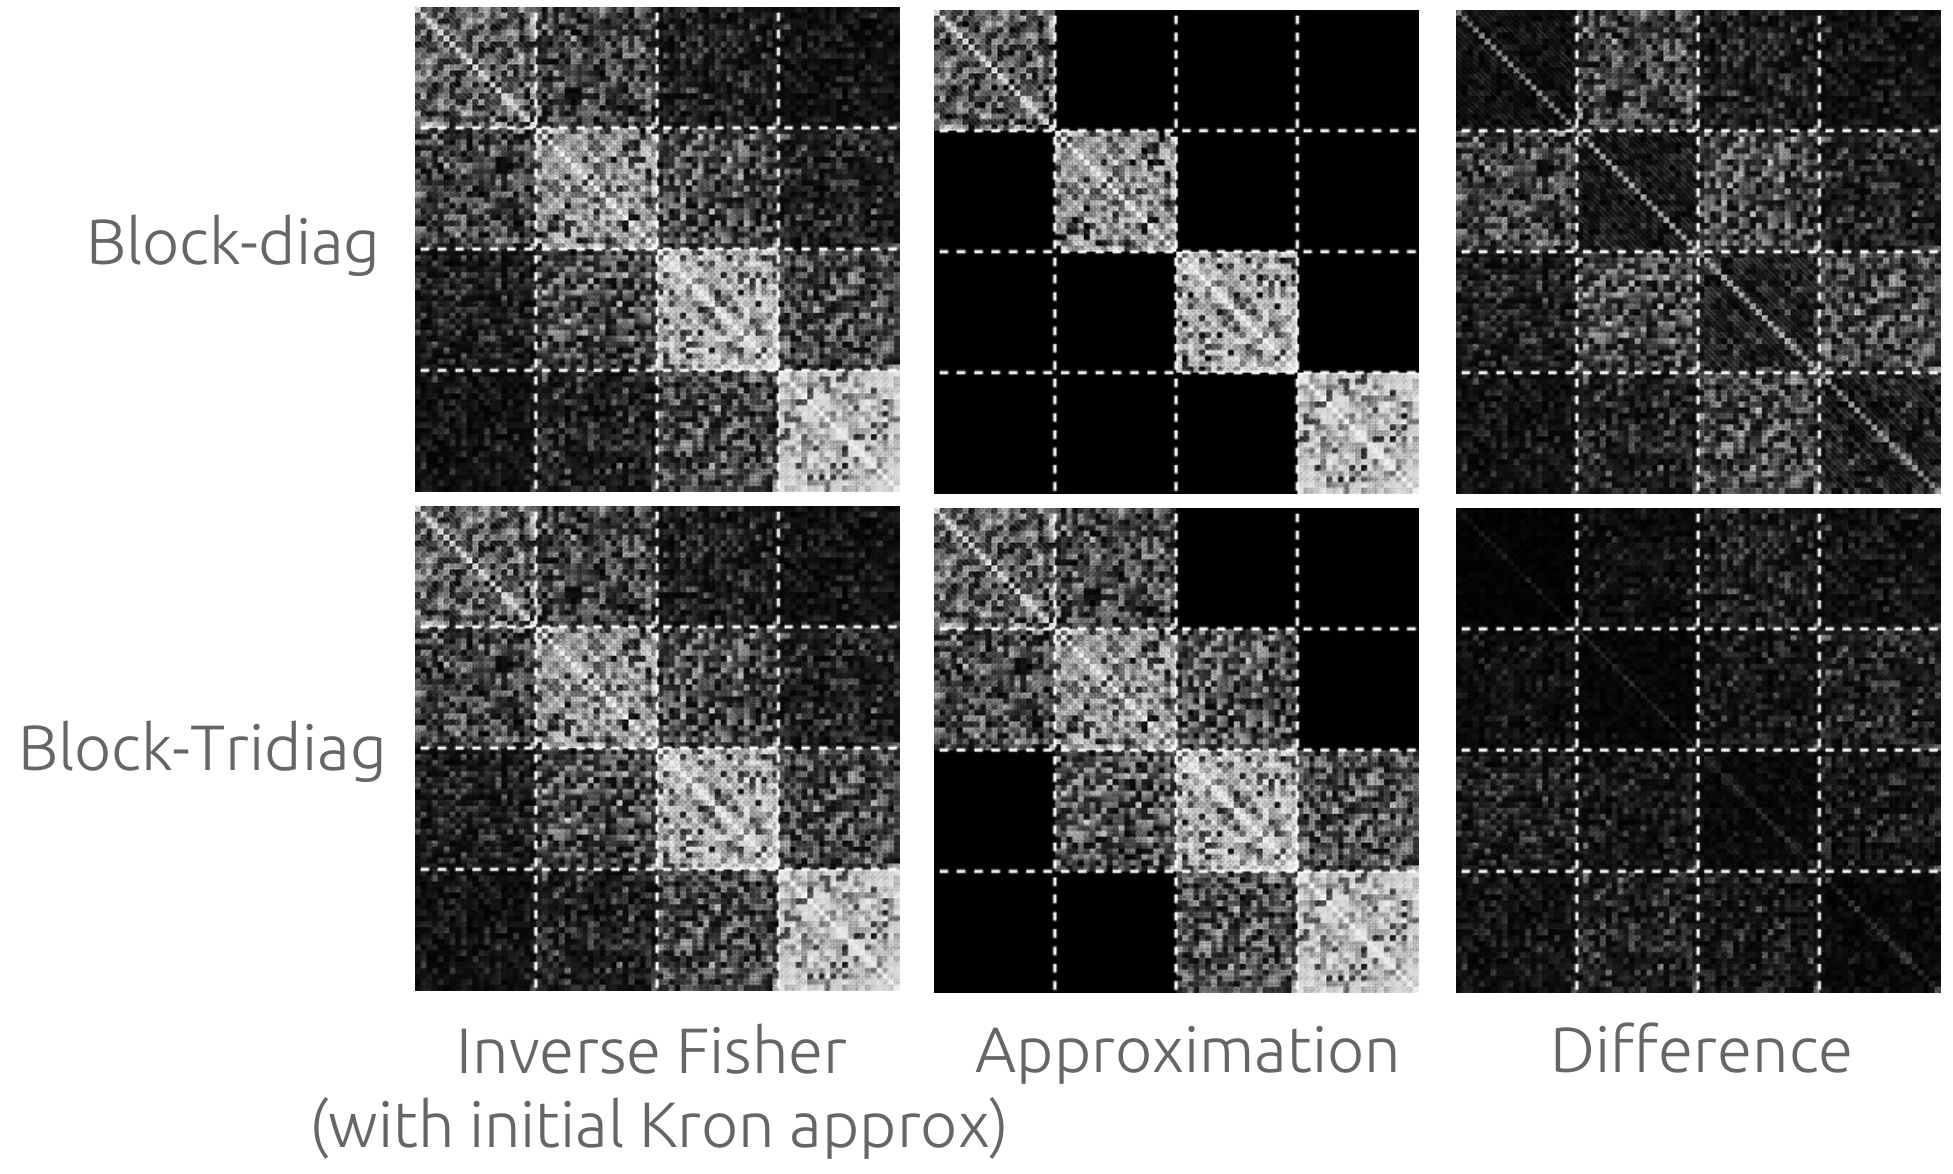
\includegraphics[scale=0.175]{kfac_12}
\end{figure}

\end{frame}

\begin{frame}
\frametitle{KFAC: Block-tridiagonal inverse approx, $\hat{F}^{-1} \approx \tilde{F}^{-1}$}
\begin{itemize}
    \item Define $\hat{F}$ to be the matrix which agrees with $\tilde{F}$ on the tridiagonal blocks, and
        which satisfies the property that $\hat{F}^{-1}$ is block-tridiagonal
    \item Assume that $\hat{F}^{-1}$ is block-tridiagonal is equivalent to
        \begin{itemize}
        \item assuming that it is the precision matrix of an undirected Gaussian graphical model (UGGM) over $\mathcal{D}\theta$
        \end{itemize}
    \item As this graphical model has a tree structure, there is an equivalent
        directed graphical model with the same distribution
        \begin{itemize}
        \item this equivalent directed model will also be linear/Gaussian, and
        \item hence, a directed Gaussian Graphical model (DGGM).
        \end{itemize}
\end{itemize}

{\footnotesize
Recall: The precision matrix of a random vector is the inverse of its covariance matrix.
% * https://www.statlect.com/glossary/precision-matrix
}
\end{frame}

\begin{frame}
\frametitle{KFAC: Block-tridiagonal inverse approx, $\hat{F}^{-1} \approx \tilde{F}^{-1}$}
\begin{figure}
    \centering
    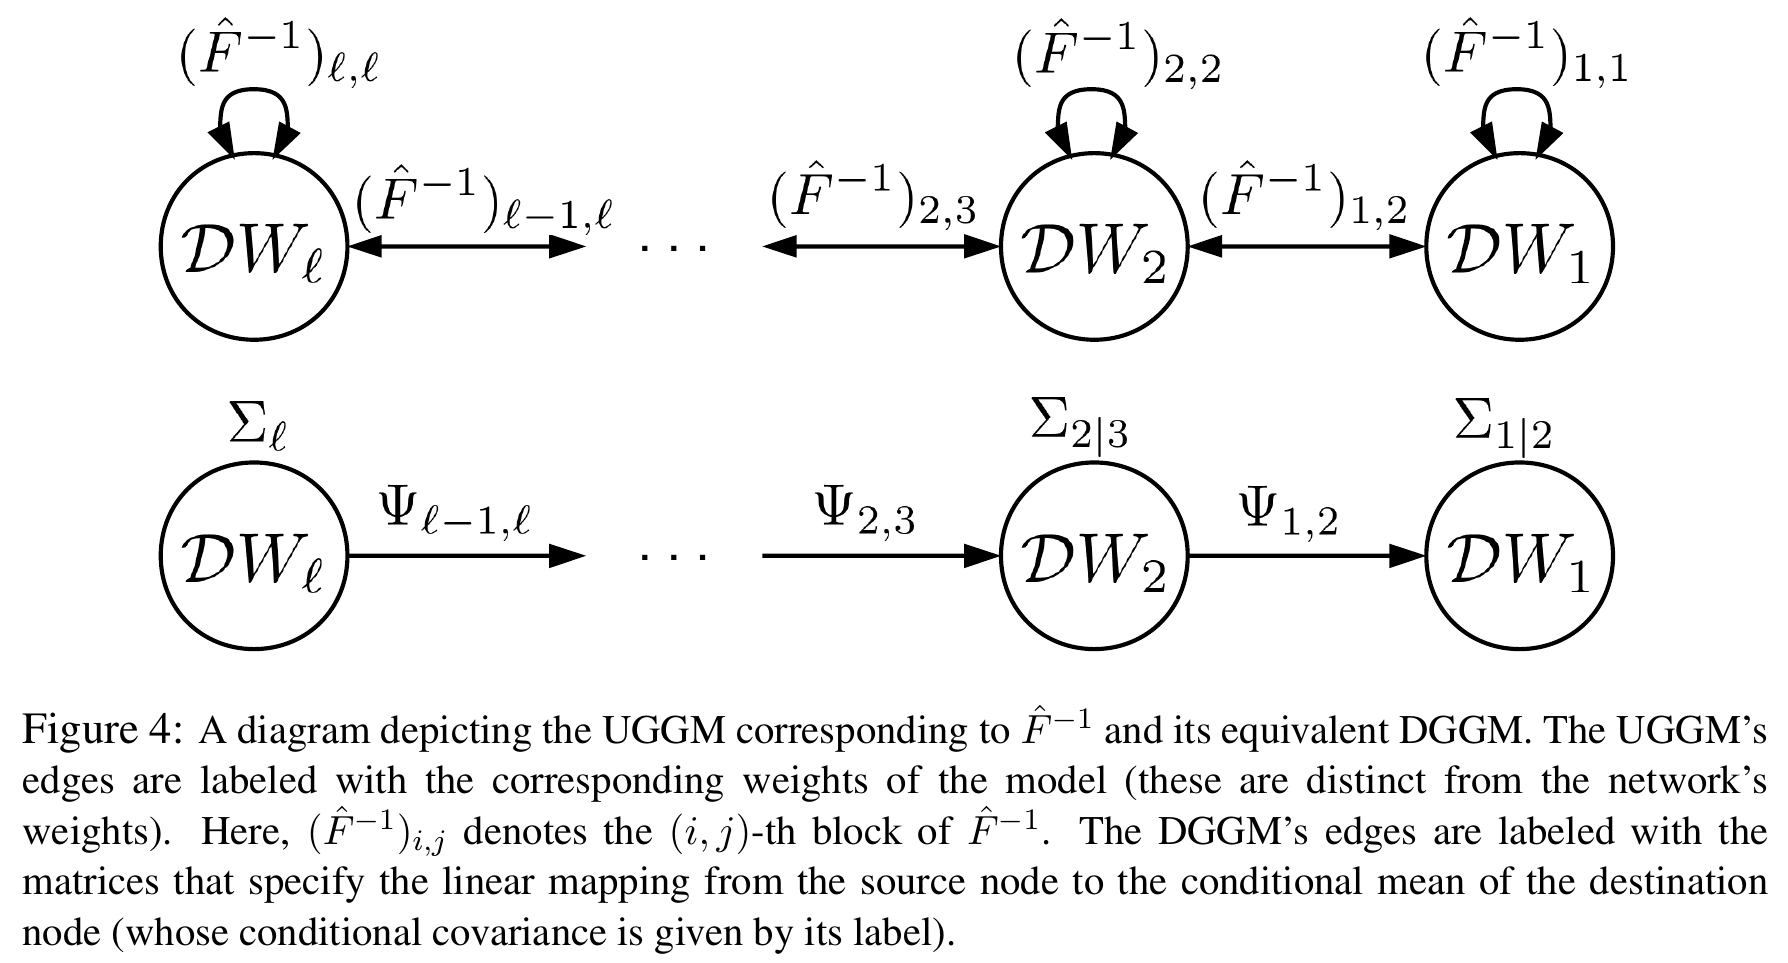
\includegraphics[scale=0.25]{kfac_fig_04_arxiv}
\end{figure}
\end{frame}

\begin{frame}
\frametitle{KFAC: Block-tridiagonal inverse approx, $\hat{F}^{-1} \approx \tilde{F}^{-1}$}
Applying formula for inverse covariance of directed model used in FActorized Natural Gradient (FANG)(Grosse and Salakhutdinov, 2015)
gives:

\begin{figure}
    \centering
    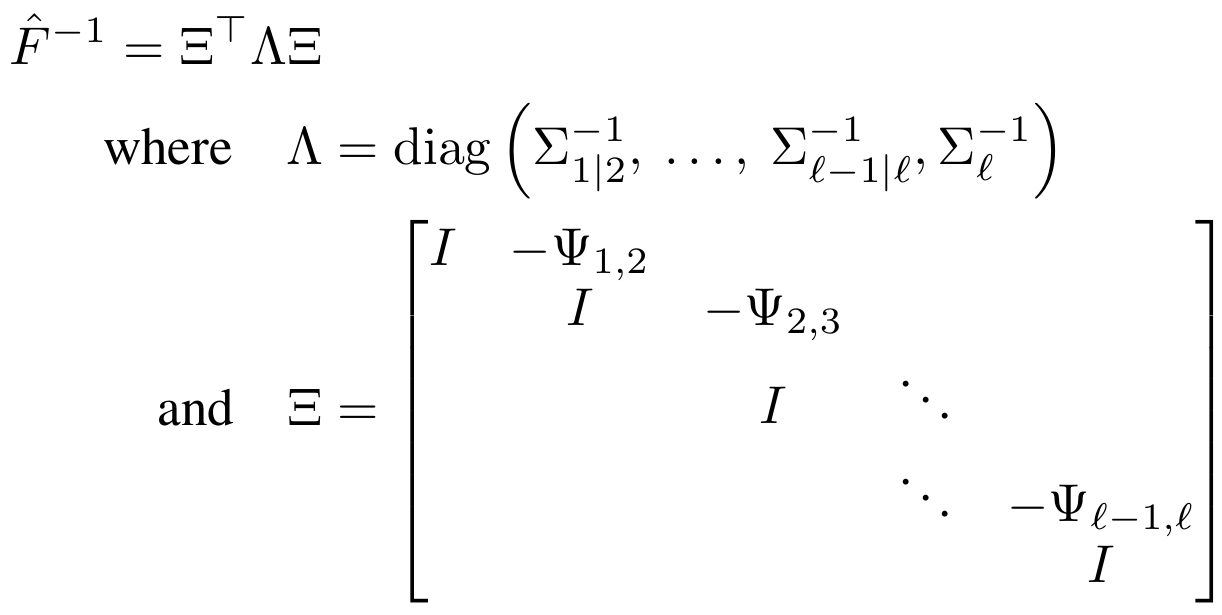
\includegraphics[scale=0.25]{kfac_14}
\end{figure}

% \begin{figure}
%     \centering
%     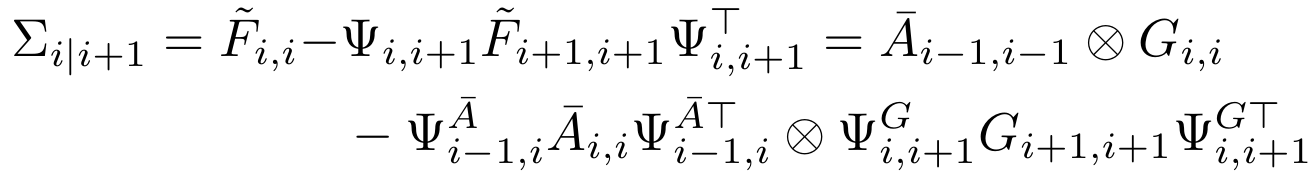
\includegraphics[scale=0.15]{kfac_15}
% \end{figure}
\end{frame}

% \begin{frame}
% \frametitle{KFAC: Block-tridiagonal inverse approx, $\hat{F}^{-1} \approx \tilde{F}^{-1}$}
% \begin{figure}
%     \centering
%     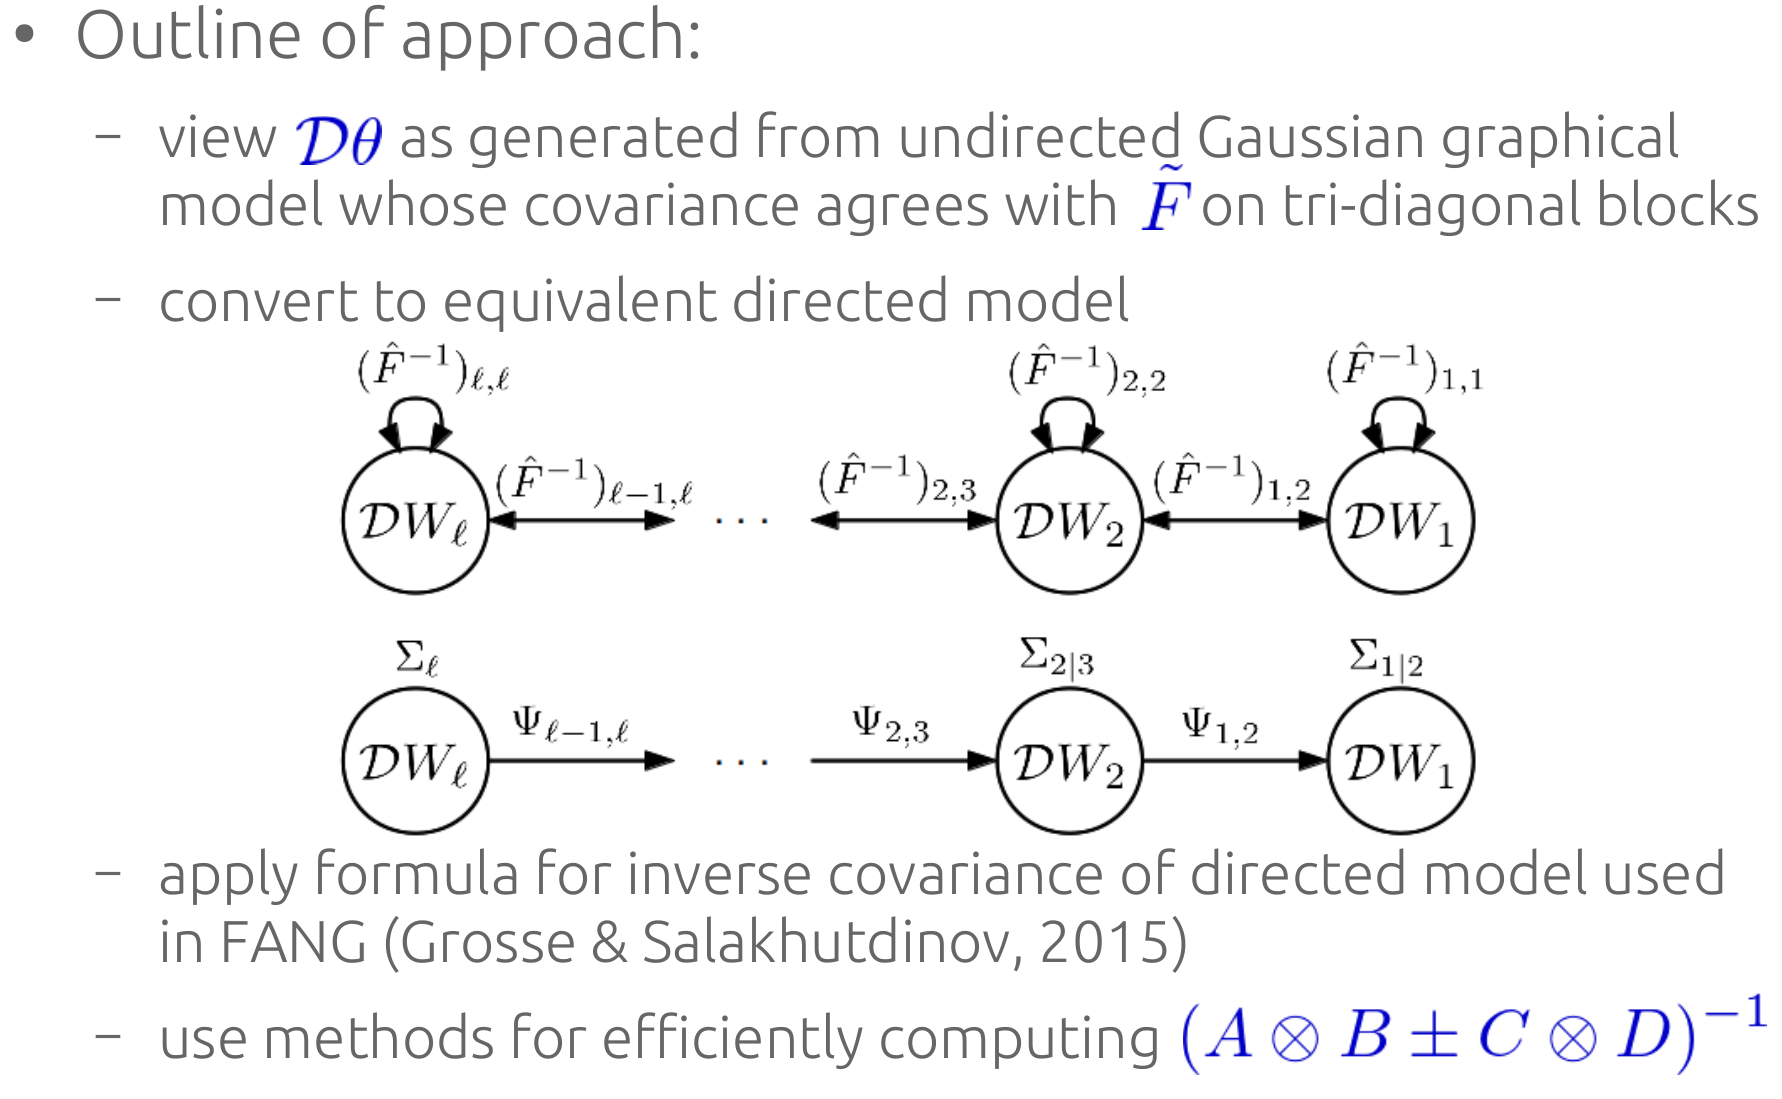
\includegraphics[scale=0.225]{kfac_11}
% \end{figure}
% \end{frame}

